\section{\Mimir\ Architecture}

\Mimir\ is divided into a number of related modules.

\begin{description}
\item[mimir-core] The core Java library to create a \Mimir\ index on disk, add
GATE documents to the index, and then query the index once it has been built.
Also provides some abstract helper classes for the annotation storage layer,
but not the actual storage implementations (which are provided by separate
plugins, leveraging the CREOLE plugin framework of GATE Embedded).

\item[plugins/db-h2] The default annotation storage implementation.  This
stores annotation data using H2\footnote{\url{http://h2database.com}}, an
in-process embedded SQL database.

\item[plugins/sesame] An alternative annotation storage implementation that
stores its annotation data in a triple store using the Sesame API
(\url{http://www.openrdf.org/}).  Annotations with an ``inst'' feature are
treated as links into the knowledge base, supporting richer semantic queries.

\item[plugins/sparql] A helper that can be layered on top of any other storage
implementation to provide semantic querying against a separate knowledge base,
accessible at a SPARQL endpoint.

\item[plugins/measurements] A special-purpose helper for Measurement
annotations created by the GATE {\tt Tagger\_Measurements} plugin.  Queries are
normalised into SI units so can retrieve annotations that express the same
measurement in different terms (e.g. an annotation for ``90 seconds'' would
match a query for ``1 to 2 minutes'').

\item[mimir-client] The client side of the \Mimir\ remote protocol, to support
distributed indexing and querying.

\item[mimir-web] A Grails\footnote{\url{http://grails.org}} plugin providing
both the user interface to create and query indexes over the web, and also the
server side of the remote protocol to expose several distributed \Mimir\
indexes as a single {\em federated} index for clients.  This is provided as a
plugin rather than an application to make it more easily customisable.

\item[mimir-cloud] An example Grails application, that uses the {\tt mimir-web}
plugin and also includes security support. This is the exact implementation used
for \Mimir{} servers supplied on the GATECloud.net
platform\footnote{\url{https://gatecloud.net}: a platform for running GATE-based
processes on the cloud.}. This application should be suitable without any
modifications for most users.
\end{description}

\section{Building and Running a \Mimir{} Web
Application}\label{sec:building}

The {\tt mimir-core} Java library provides support for indexes that are
represented as an on-disk directory -- named {\em Local Indexes} in the rest of
this document (see the discussion about index types in
Section~\ref{sec:admin:index-types}). To get the full functionality of \Mimir{}
(including support for {\em Remote} and {\em Federated} indexes, as well as user
interfaces for system administration and searching indexes) you will need to
build and run a web application. All the web elements of \Mimir{} are
implemented as the {\tt mimir-web} Grails plugin, which can easily be included
in any Grails-based web application. The standard \Mimir{} distribution provides
such a web application, named {\tt mimir-cloud}.

\subsection{The {\tt mimir-cloud} Web Application}
\label{sec:mimir-cloud}
The {\tt mimir-cloud} web application is the actual version of the \Mimir\
software that is used on the GATECloud platform. As such, it is configured for
that particular usage scenario, where indexes have two different URLs (depending
on whether they are accessed from within the same cloud region or not), and
where the local configuration page is not made available to the user. However,
some of this behaviour is switched off when the application detects that it is
not running on the cloud, to allow it to be used as a general purpose
\Mimir{}-enabled web application.

In addition to the {\tt mimir-web} plugin, it also includes some basic support
for user authentication (using the Spring Security Grails plugin), and support
for packaging and downloading local indexes. This is probably a suitable choice
if you just need a stand-alone web application with \Mimir{} functionality, and
you do not intend to develop your own security solution.

If you are an experienced Grails developer and you intend to add your own
security solution, then you should use the {\tt mimir-web} Grails plugin
directly in your own application, as described in
Section~\ref{sec:extend:customapp}.

While we include this application as an example of a fully-fledged Grails
application using the {\tt mimir-web} plugin, you may need to modify it slightly
to make it mode suitable to your actual usage scenario.

\subsection{Prerequisites}

To build the \Mimir\ web application you will need:
\begin{itemize}
\item A Java 6 JDK.  \Mimir\ has been tested with the Sun/Oracle and OpenJDK
  JVMs on Linux and the Apple JVM on Mac OS X.
\item Apache Ant 1.8.1 or later.
\item The Grails framework:  the \Mimir\ plugin was developed using Grails
  version 2.1.3. Other versions of Grails are not guaranteed to work, so you
  should use the same one. You need to set the JAVA\_HOME environment variable
  to  point to your JDK, the GRAILS\_HOME environment variable to point to your
  Grails installation and add \$GRAILS\_HOME/bin to your PATH.
\end{itemize}

While not strictly a pre-requisite, \Mimir\ performs much better on 64-bit
systems than on 32-bit ones, partly due to simply being able to assign more
memory to the process, but also because the larger address space allows MG4J to
memory-map many of the files that make up the index.

To run a local instance of \Mimir\ you can use the standard \cmd{grails prod
run-war} command, but to deploy a production instance you will need a separate
servlet container such as Tomcat.

\subsection{Building}

There is a top-level Ant build.xml file that should build all the modules in
the correct order. To do that simply change to the top level directory
containing the \Mimir\ source code, and run the \cmd{ant} command. To perform
the same build process manually, you need to change to the following directories
and run the following {\tt ant} commands in this order:
\begin{enumerate}
\item {\tt mimir-core}: \cmd{ant publish}
\item {\tt mimir-client}: \cmd{ant publish}
\item {\tt plugins}: run \cmd{ant} in each sub-directory of the plugins
  directory in turn (order is not important here, the plugins do not depend on
  one another).
\item {\tt mimir-web}: \cmd{grails compile} followed by \cmd{grails
  compile-gwt-modules}.
\end{enumerate}

The next step is to configure the {\tt mimir-cloud} web application, and is
described in the following Section.

\subsection{Configuring}\label{sec:admin:config}

When the \Mimir\ Grails plugin is installed into a Grails application, it
creates a base configuration file at {\tt grails-app/conf/MimirConfig.groovy}.
This file contains a number of settings that affect the running of the \Mimir\
components. In many cases the default options will be sufficient, but you should
nevertheless check the configuration and make sure it is appropriate for your
needs.

\begin{lstlisting}
gateInit {
  gateHome = "WEB-INF/gate-home"
  userConfigFile = "WEB-INF/gate-home/user.xml"
}
\end{lstlisting}

Since \Mimir\ is based on GATE, the plugin initialises the GATE environment at
start-up.  These parameters control the initialisation process.  In most cases
you can leave the values at their defaults, which use a deliberately cut-down
set of GATE configuration files installed into {\tt web-app/WEB-INF} by the
\Mimir\ Grails plugin.  The available parameters are gateHome, pluginsHome,
siteConfigFile, userConfigFile and builtinCreoleDir, which correspond to the
standard settings on the
\htlink{http://hudson.gate.ac.uk/job/GATE-Nightly/javadoc/gate/Gate.html}{Gate}
class, and their values can be either absolute URLs (such as
\verb|file:/opt/gate|) or paths which are taken relative to the web application
(i.e. the web-app directory of the Grails application).

\begin{lstlisting}
plugins {
  h2 = "../plugins/db-h2"
  myCustomPlugin = "file:/data/mimir/plugins/myCustomPlugin"
}
\end{lstlisting}

This section specifies the \Mimir\ plugins that should be loaded, and
determines the kinds of annotation helpers you will be able to use in your
indexes.  You generally need at least one of the standard {\tt db-h2} and/or
{\tt sesame} plugins to be able to do anything useful with \Mimir, and you may
want the {\tt measurements} plugin as well if you will be searching on
Measurement annotations and/or the {\tt sparql} plugin if you have an external
knowledge base.  Section~\ref{sec:indexing:helpers} has more information about
the standard annotation helpers, and section~\ref{sec:extend:helpers} discusses
how to implement your own custom ones.

\Mimir\ uses the GATE plugin mechanism, so \Mimir\ plugins are actually
very simple CREOLE plugins\footnote{See
\url{http://gate.ac.uk/userguide/chap:creole-model}.}, used to add a set of
{\tt jar} files to the current classpath.
 
Plugins can be specified either as absolute URLs or as paths relative to the
Grails application base directory.  Absolute URLs will be loaded as such both
in {\tt run-app} and in WAR deployments, but plugins specified as relative
paths are treated slightly differently.  They will be loaded directly from the
specified paths in {\tt run-app}, but when building a WAR file the referenced
plugins will be packaged inside the WAR file and loaded from there at run-time.

\begin{lstlisting}
queryTokeniserGapp = 
    "WEB-INF/gate-home/default-query-tokeniser.xgapp"
\end{lstlisting}

Whereas GATE's usual data model deals with annotations in terms of their {\em
character} offsets from the start of the document, \Mimir\ deals in terms of
{\em tokens}.  Queries for plain text strings in \Mimir\ must be tokenised
before they can be matched against the index, and the tokenisation applied to
the queries must match that applied to the documents that have been indexed.
The \Mimir\ Grails plugin uses a saved GATE application state (gapp file) to
perform query tokenisation, the location of which is specified here.  Again,
the location can be an absolute URL or a path relative to the web-app
directory, and the default value refers to a simple app installed by the
\Mimir\ Grails plugin that contains a single ANNIE tokeniser with its default
settings.

If your tokenisation requirements are more complex, you can provide your own
saved application, or alternatively you can use your application's {\tt
resources.xml} or {\tt resources.groovy} to override the definition of the
Spring bean named ``queryTokeniser'' -- this bean must define a GATE
LanguageAnalyser that will produce annotations of type Token in the default
annotation set.

Note that because of the special handling at build time of plugins referenced
as relative paths (see above), if you want to load additional plugins into a
WAR-packaged \Mimir\ using run-time settings in an external configuration file,
then the plugins must be specified using absolute URLs, i.e.
{\tt gate.mimir.plugins.custom = "file:/opt/mimir/plugins/custom"}.  Relative
plugin paths are ignored at run-time by \Mimir\ when running from a WAR
deployment.  However, since \Mimir\ plugins are simply standard GATE CREOLE
plugins and the \Mimir\ Grails plugin initialises GATE Embedded using Spring
you can load extra plugins relative to your web app by using Spring
configuration in {\tt WEB-INF/spring/resources.xml} (see
\url{http://gate.ac.uk/userguide/sec:api:spring} for details):

\begin{lstlisting}
<beans xmlns="http://www.springframework.org/schema/beans"
    xmlns:gate="http://gate.ac.uk/ns/spring"
    xmlns:xsi="http://www.w3.org/2001/XMLSchema-instance"
    xsi:schemaLocation="
      http://www.springframework.org/schema/beans
      http://www.springframework.org/schema/beans/spring-beans.xsd
      http://gate.ac.uk/ns/spring
      http://gate.ac.uk/ns/spring.xsd">
  <gate:extra-plugin>WEB-INF/custom-plugin</gate:extra-plugin>
</beans>
\end{lstlisting}

\subsection{Running}

The easiest way to run the \Mimir\ cloud web app is to use the normal Grails
commands \cmd{grails run-app} or \cmd{grails run-war}.  For performance,
\cmd{grails prod run-war} is preferable.  For anything more than the smallest
toy index it is advisable to increase the memory available to \Mimir\ by using
the JAVA\_OPTS environment variable.  For example (using bash or a similar POSIX
shell):
\begin{verbatim}
$ JAVA_OPTS='-Xmx4G' grails prod run-war
\end{verbatim}

To shut down a web app started using \cmd{grails run-app} or \cmd{grails
run-war}, simply create an empty file in the {\tt mimir-cloud} directory named
``{\tt .kill-run-app}''.  Grails watches for this file and will shut down
gracefully when it detects that the file has been created.

For production deployments, a better option is to build a WAR file using
{\tt grails prod war} and deploy that to a standalone servlet container such as
Apache Tomcat.  If you are using Ubuntu or Debian GNU/Linux, it is better to
download the standard Tomcat ZIP package from Apache and use that rather than
installing the Tomcat available through {\tt apt-get} as the latter is
configured by default with a security manager that interferes with \Mimir.

When deployed to a servlet container the web application reads configuration
at run-time from two locations using the Grails standard ``externalised
configuration'' mechanism:
\begin{itemize}
\item {\tt WEB-INF/classes/mimir-app-config.groovy} inside the web application.
\item {\tt mimir-config.groovy} in the working directory of the Java process.
\end{itemize}

Any values in these files override values specified in {\tt MimirConfig.groovy}
or the main application {\tt Config.groovy}.  For production deployments, you
should be sure to specify the public URL of your \Mimir\ server in one of these
configuration files.  For example:
\begin{lstlisting}[texcl]
gate.mimir.indexBaseDirectory = "/data/mimir/indexes"
grails.serverURL = "http://example.com/mimir"
// or just http://example.com if you have deployed \Mimir
// as the ROOT web application
\end{lstlisting}

%%%%%%%%%%%%%%%%%%%%%%%%%%%%%%%%%%%%%%%%%%%%%%%%%%%%%%%%%%%%%%%%%%%%%%%%%%%%%%
\section{Indexes in \Mimir}

\subsection{Types of Index}\label{sec:admin:index-types}

A single instance of \Mimir\ can host several indexes.  \Mimir\ supports
{\em local} indexes, stored in the file system of the \Mimir\ server, and
{\em remote} indexes, which are a view of an index hosted in another \Mimir\
instance (possibly on a different machine).  Several indexes (of any type) can
be combined into a {\em federated} index, which presents the group of indexes as
a single virtual index.  All the indexing and searching functionality of
\Mimir\ applies equally to all three index types.

Each \Mimir\ index has a {\em state}, and the operations that can be performed
on the index depend on which state it is currently in.  When first created, a
local index will be in the {\em indexing} state, meaning it is waiting for
documents to be added to the index.  When all the documents have been added to
the index an administrator will close the index, putting it into the {\em
closing} state.  For large indexes the closing process can take several hours,
and when it is complete the index will enter the {\em searching} state, at
which point it is available for querying.  The other possible state for a local
index is {\em failed}, indicating a problem with the index.  Typically a failed
index will need to be deleted by the administrator.  Thus it is apparent that
an index cannot be used simultaneously for searching and indexing.  An existing
set of index files can be imported into a running \Mimir\ instance as a local
index, which will then immediately be in the {\em searching} state.

Remote indexes inherit their state from the remote server, and federated
indexes inherit their state by combining the states of their component indexes.
A federated index may occasionally appear in the {\em working} state if its
component indexes are not all in the same state (for example if some of them
have started closing but others are still in {\em indexing} mode), but the
working state will usually resolve to a normal state once the component indexes
have synchronised.

Note that once a local index has moved from {\em indexing} to {\em closing} to
{\em searching} it is not possible to add more documents to the same index.
The suggested way to add to an index is to create a new index to hold the new
documents, fill it, close it, and then create a federated index consisting of
the original index plus the new one (or if the original index was itself
federated, add the new index to the existing federation).

A typical setup for a large-scale indexing task would be to have a number of
identical ``slave'' servers running \Mimir, each with a single local index.  A
single ``master'' \Mimir\ instance could then have one remote index definition
pointing to each of the slaves, and a single federated index combining the
remote indexes.  This federated index would be the point of entry into the
system and would share out indexing jobs (round-robin among the slaves) or
search requests (to all the slaves in parallel) as appropriate.

\subsection{Creating a Local Index}

Indexes in \Mimir\ are managed through the web interface.  The front page of a
newly-installed \Mimir\ is shown in Figure~\ref{fig:front-page}.
%
\begin{figure}[htb!]
\begin{center}
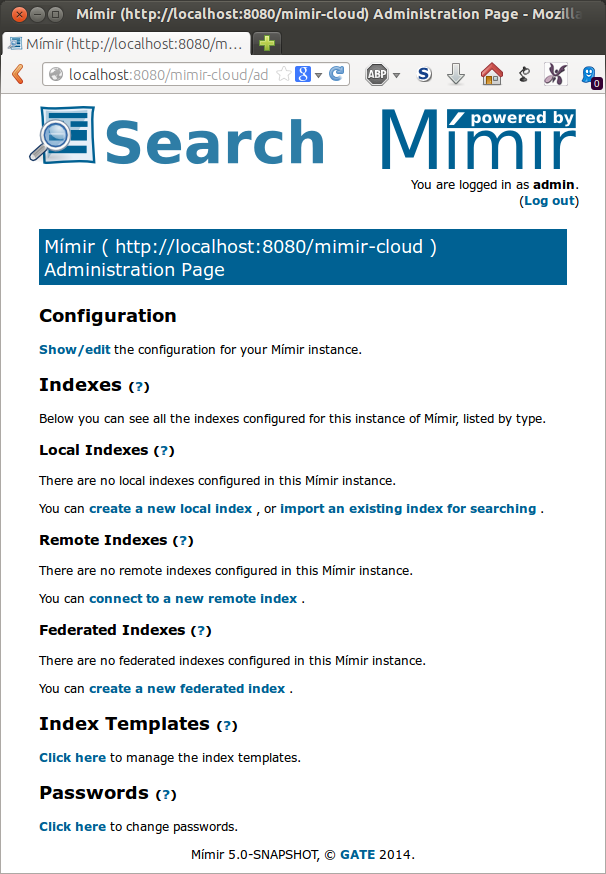
\includegraphics[scale=0.5]{img/default-front-page}
\end{center}
\caption{The default front page of a new \Mimir}
\label{fig:front-page}
\end{figure}
%
The {\em index templates} mentioned at the bottom, are used to define the
properties of new indexes, and are described in more detail in
Chapter~\ref{sec:indexing}.  The \Mimir\ Grails plugin provides a single
example template based on ANNIE annotation types.

To create an empty local index ready to receive documents for indexing, select
the {\em create a new local index} link.  This will present a form
(Figure~\ref{fig:new-local-index}) asking for the name of the new index and the
template from which it should be created.  The ``Document URIs are external
links'' option affects the way documents are presented in the search interface.
Every document in \Mimir\ is identified by a URI, and if you intend to use
document URIs that are actually resolvable URLs (for example if your documents
came from a web crawl) then you should select this option to add a link to the
original document to the search results.  If the document URIs will not be
resolvable URLs then leave the option un-selected.
%
\begin{figure}[htb!]
\begin{center}
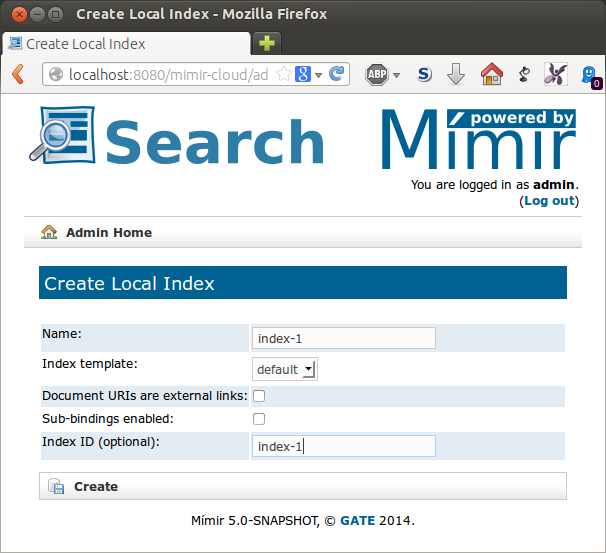
\includegraphics[scale=0.5]{img/new-local-index}
\end{center}
\caption{Creating a new local index}
\label{fig:new-local-index}
\end{figure}
%
The index will be assigned a unique identifier and a new directory will be
created under the \verb|indexBaseDirectory| you configured earlier to
hold the index data.  The newly-created index will be in the {\em indexing}
state (see Figure~\ref{fig:local-index-created}), ready to receive documents
for indexing.  For details of how to submit documents to the index, see
Chapter~\ref{sec:indexing}.
%
\begin{figure}[htb!]
\begin{center}
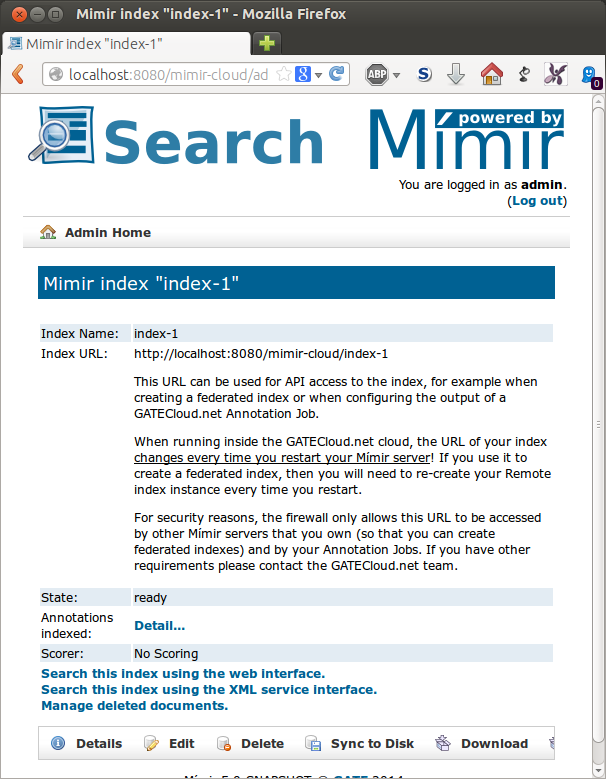
\includegraphics[scale=0.5]{img/local-index-created}
\end{center}
\caption{Results of creating a new local index}
\label{fig:local-index-created}
\end{figure}
%

This {\em index information} page can be accessed at any time by clicking the
link for the relevant index name from the \Mimir\ front page
(Figure~\ref{fig:local-index-list}).
%
\begin{figure}[htb!]
\begin{center}
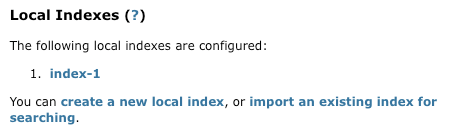
\includegraphics[scale=0.5]{img/local-index-list}
\end{center}
\caption{List of local indexes on the \Mimir\ front page}
\label{fig:local-index-list}
\end{figure}
%
Once all the documents to be indexed have been submitted the index can be
closed using the {\em Close} link on the index information page.  This will
change the state of the index to {\em closing} as described above and begin the
closing process.  The information page will show a live-updating progress bar
(Figure~\ref{fig:local-index-closing}) giving some indication of the time
remaining until the index has completely closed.
%
\begin{figure}[htb!]
\begin{center}
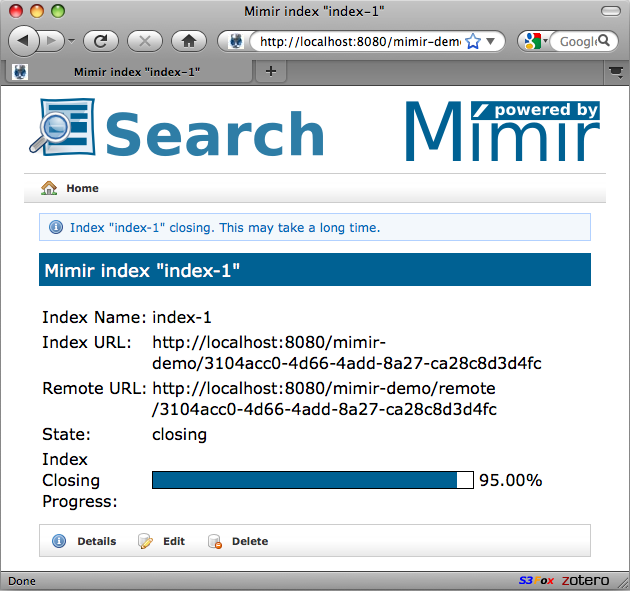
\includegraphics[scale=0.5]{img/local-index-closing}
\end{center}
\caption{Closing a local index}
\label{fig:local-index-closing}
\end{figure}
%

When the closing process is complete (the progress bar reaches 100\%) the index
will switch into {\em searching} mode, and the index can then be searched using
the tools described in Chapter~\ref{sec:searching}.

\subsection{Working with Remote and Federated Indexes}

The architecture of \Mimir\ is designed to make working with remote and
federated indexes as transparent as possible.  The setup process will obviously
vary for the different index types, but once created the process of submitting
documents for indexing or of performing queries is exactly the same for all
indexes.

\subsubsection{Remote indexes}\label{sec:admin:remote-index}
A {\em remote} index is a mechanism whereby one \Mimir\ instance can
transparently index documents in, or send queries to, an index that is located
in a different \Mimir\ instance, typically running on separate hardware.  To
connect one {\em master} \Mimir\ instance to an index running in another {\em
slave} instance, first visit the index information page for the relevant
index on the slave and make a note of its {\em remote URL} (typically a URL of
the form \verb|http://server:port/mimir/remote/{UUID}|).  Now on the front page
of the master instance, select the {\em connect to a new remote index} link.
This will present a form (Figure~\ref{fig:connect-remote-index}) asking for a
name for the remote index (which need not be the same as the name of the index
on the slave), and a {\em remote URL} which is the one you made a note of from
the slave above. You should never create a remote index pointing to another
index in the same \Mimir\ instance. Such a configuration is not supported and
will lead to errors!
\begin{figure}[htb!]
\begin{center}
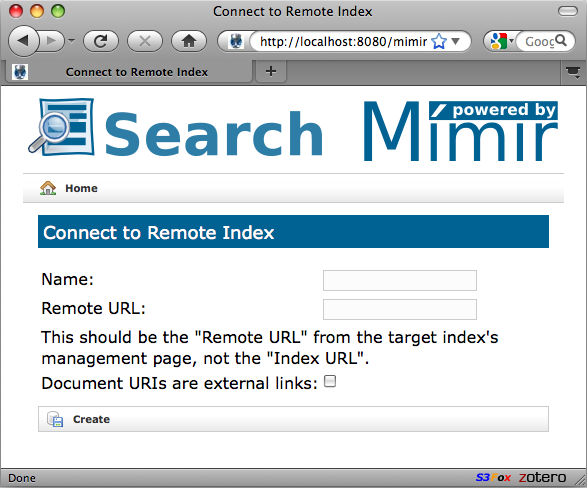
\includegraphics[scale=0.5]{img/connect-remote-index}
\end{center}
\caption{Connecting to a remote index}
\label{fig:connect-remote-index}
\end{figure}
%

The remote index defined on the master server will synchronise its state with
that of the underlying index on the slave, and once created will be usable
exactly like a local index.  However remote indexes are rarely used directly,
as in most cases it is more efficient to operate on the slave instance
itself.  The main benefit of remote indexes comes when they are used as part
of a {\em federated index}.

\subsubsection{Federated indexes}

A {\em federated index} is a device to bundle several indexes (which can
themselves be local, remote or federated) together so they can be used as a
single index.  Documents for indexing are shared out between the component
{\em sub-indexes}, and searches are performed by all sub-indexes in parallel.
Thus a federation of five indexes each containing 200,000 documents will
typically run queries faster than a single index containing 1 million
documents.  To create a federated index, go to the \Mimir\ front page and
select the {\em create a new federated index} link.  This will present a form
(Figure~\ref{fig:new-federated-index}) asking for a name for the federated
index.  The form also includes a multiple-selection list to specify the
sub-indexes to be included in the federated index.  Select the appropriate
entries from this list using the usual multiple list selection mechanism
(ctrl-click on Windows or Linux, cmd-click on Mac OS X) and press the
{\em Create} button to create the index.
%
\begin{figure}[htb!]
\begin{center}
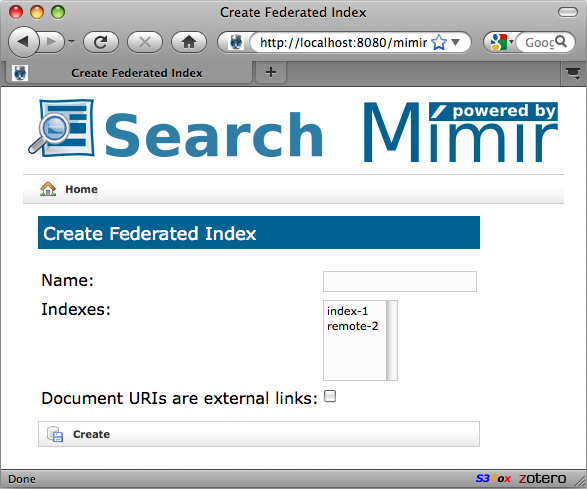
\includegraphics[scale=0.5]{img/new-federated-index}
\end{center}
\caption{Creating a new federated index}
\label{fig:new-federated-index}
\end{figure}
%
Once created the federated index will be usable exactly like a local or remote
index.

\subsection{Deleting Indexes}

If an index registered with Mimir is no longer required it can be deleted by
selecting the {\em Delete} button from the index information page (accessible
by clicking on the name of the relevant index on the \Mimir\ front page).  For
remote and federated indexes this simply deletes the ``registration'' of the
index with \Mimir, which can be easily re-created as above.  For local indexes
it also offers the option to delete the underlying index files from disk.  If a
local index in {\em searching} state is deleted without deleting the disk files
then the index can be re-created later using the {\em import an existing index
for searching} option from the \Mimir\ front page.  However, if a local index
in the {\em indexing} or {\em closing} state is deleted without having been
properly closed then the index files will be unusable and will need to be
deleted manually.

\Mimir\ will not allow the deletion of an index which is currently part of a
federated index in the same \Mimir\ instance.  To delete such an index, it must
first be removed from the federated index.  This guarantee only applies to
indexes within a {\em single} \Mimir\ instance --- \Mimir\ does not prevent the
deletion of an index on a slave instance which is being used as a remote index
by a master instance (it prevents the deletion of the remote index definition
in the master but not the slave index it points to).  However to do so would
put the remote index on the master (and hence any federated index that it is
part of) into the {\em failed} state, preventing further use until the problem
is resolved.

\section{``Deleting'' Documents from a \Mimir\ Index}\label{sec:admin:takedown}

While \Mimir\ indexes are not directly modifiable once they have been created,
there are situations in which it is necessary to remove documents that should
not have been indexed in the first place, or documents that may be considered
libellous, etc.  To support this, \Mimir\ provides a mechanism to mark
individual documents in the index as ``deleted'', and any documents so marked
will be excluded from future queries.  It is not possible to completely delete
the data from the index files on disk, short of completely re-building the
index from scratch, but documents marked as deleted are not accessible through
any of the public \Mimir\ APIs or user interfaces.

To mark a document as deleted (or to remove an existing deletion marker, making
the document available for queries again), use the ``Manage deleted documents''
link from the index's administration page.  This will present the screen shown
in figure~\ref{fig:deleted-documents}, with a text box into which you can type
one or more (space-separated) document IDs, and choose whether to mark them as
deleted or as ``not deleted'' (i.e. to remove any existing deletion markers for
those document IDs).
%
\begin{figure}[htb!]
\begin{center}
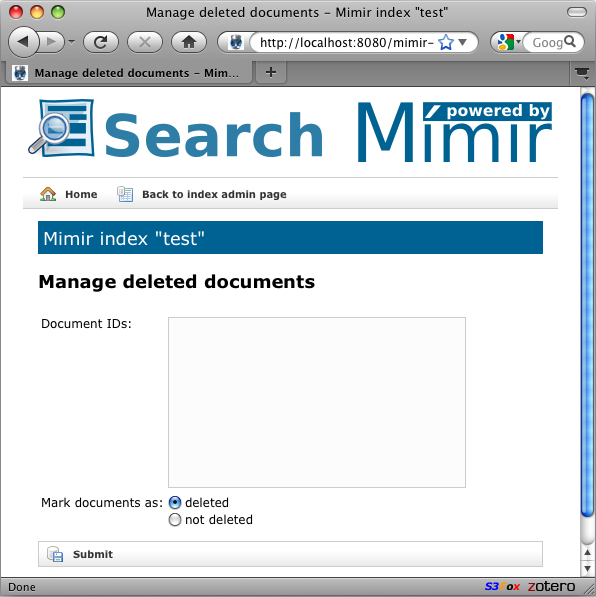
\includegraphics[scale=0.5]{img/deleted-documents}
\end{center}
\caption{Managing deleted documents}
\label{fig:deleted-documents}
\end{figure}

Note that the IDs required here are not the URIs that were provided with the
documents when they were indexed, but the internal \Mimir\ document IDs which
are numbers starting from 0, as returned in the hit lists and ``getDocumentId''
by the \Mimir\ query APIs (see section~\ref{sec:search:service}).